\documentclass[
	letterpaper,
	a4paper,
	cleardoublepage=empty,
	headings=twolinechapter,
	numbers=autoenddot,
]{article}
\usepackage{amsmath}
\usepackage{cancel}
\usepackage{amsfonts}
\usepackage{amssymb}
\usepackage{tikz}
\usepackage{epigraph}
\usepackage{import}
\usepackage{float}
\usepackage{hyperref}

\usepackage{todonotes}
\usepackage{verbatim}
\usepackage{caption}
\usepackage{subcaption}

\newcommand{\Fig}[0]{Fig.}
\newcommand{\Eq}[0]{Eq.}

\renewcommand\epigraphflush{flushright}
\renewcommand\epigraphsize{\normalsize}
\setlength\epigraphwidth{0.7\textwidth}

\definecolor{titlepagecolor}{cmyk}{1,.60,0,.40}

\DeclareMathOperator*{\argmax}{argmax}
\DeclareFixedFont{\titlefont}{T1}{ppl}{b}{it}{0.5in}

\makeatletter                       
\def\printauthor{%                  
	{\large \@author}}              
\makeatother
\author{
	Wasim Essbai
}

\newcommand\titlepagedecoration{%
	\begin{tikzpicture}[remember picture,overlay,shorten >= -10pt]
		
		\coordinate (aux1) at ([yshift=-15pt]current page.north east);
		\coordinate (aux2) at ([yshift=-410pt]current page.north east);
		\coordinate (aux3) at ([xshift=-4.5cm]current page.north east);
		\coordinate (aux4) at ([yshift=-150pt]current page.north east);
		
		\begin{scope}[titlepagecolor!40,line width=12pt,rounded corners=12pt]
			\draw
			(aux1) -- coordinate (a)
			++(225:5) --
			++(-45:5.1) coordinate (b);
			\draw[shorten <= -10pt]
			(aux3) --
			(a) --
			(aux1);
			\draw[opacity=0.6,titlepagecolor,shorten <= -10pt]
			(b) --
			++(225:2.2) --
			++(-45:2.2);
		\end{scope}
		\draw[titlepagecolor,line width=8pt,rounded corners=8pt,shorten <= -10pt]
		(aux4) --
		++(225:0.8) --
		++(-45:0.8);
		\begin{scope}[titlepagecolor!70,line width=6pt,rounded corners=8pt]
			\draw[shorten <= -10pt]
			(aux2) --
			++(225:3) coordinate[pos=0.45] (c) --
			++(-45:3.1);
			\draw
			(aux2) --
			(c) --
			++(135:2.5) --
			++(45:2.5) --
			++(-45:2.5) coordinate[pos=0.3] (d);   
			\draw 
			(d) -- +(45:1);
		\end{scope}
	\end{tikzpicture}%
}

\begin{document}
	\begin{titlepage}
		
		\noindent
		\titlefont Report1 tesi\par
		\epigraph{Data processing, sviluppo ANN, BNN e prima analisi.}
		\null\vfill
		\vspace*{1cm}
		\noindent
		\hfill
		\begin{minipage}{0.35\linewidth}
			\begin{flushright}
				\printauthor
			\end{flushright}
		\end{minipage}
		%
		\begin{minipage}{0.02\linewidth}
			\rule{1pt}{125pt}
		\end{minipage}
		\titlepagedecoration
	\end{titlepage}

	\tableofcontents
	\pagebreak
	
	\section{Dataset}
	\subsection{Sorgente}
	Come anticipato, il dataset usato è una raccolta di segnali PPG,ECG e ABP reperibile a questo link \href{https://archive.ics.uci.edu/ml/datasets/Cuff-Less+Blood+Pressure+Estimation#}{dataset}. Questo dataset in realtà è derivato da uno più grande che si chiama MIMIC I (circa 23GB) attraverso un processing e pulizie di vario genere (descritti in un paper che c'è nella pagina del link). Ora c'è addirittura MIMIC III che arriva 2.4T. Sono dataset molto grandi perché contengono rilevamenti su diversi pazienti (circa 10000 nel III) in diverse condizioni fisiche e di salute. 
	
	Siccome la tesi non è lo sviluppo di una rete in grado di stimare la pressione sanguigna ho usato il dataset del link che è pulito e soprattutto di dimensioni ridotte.
	
	\subsection{Elaborazione}
	Dal dataset scelto poi c'era bisogno di estrarre le features dai segnali, perché una predizione puntuale è sia inutile che poco fattibile.
	
	Prima però di estrarre le features è stato necessario fare ulteriori pulizie sul dataset, che è pulito ma non abbastanza. Questo perchè il dataset era stato pensato per usare sia PPG che ECG insieme per predirre la pressione, probabilmente per loro andava bene così. Le pulizie sono state principalmente filtraggio e rilevamento di segnali dove non si riescono a rilvare i picchi. Poi ho preso segnali di durata minima pari a 2 minuti e massima a 7. Un esempio di record è in figura ~\ref{fig:data_sample}
	
	\begin{figure}[h]
		\centering
		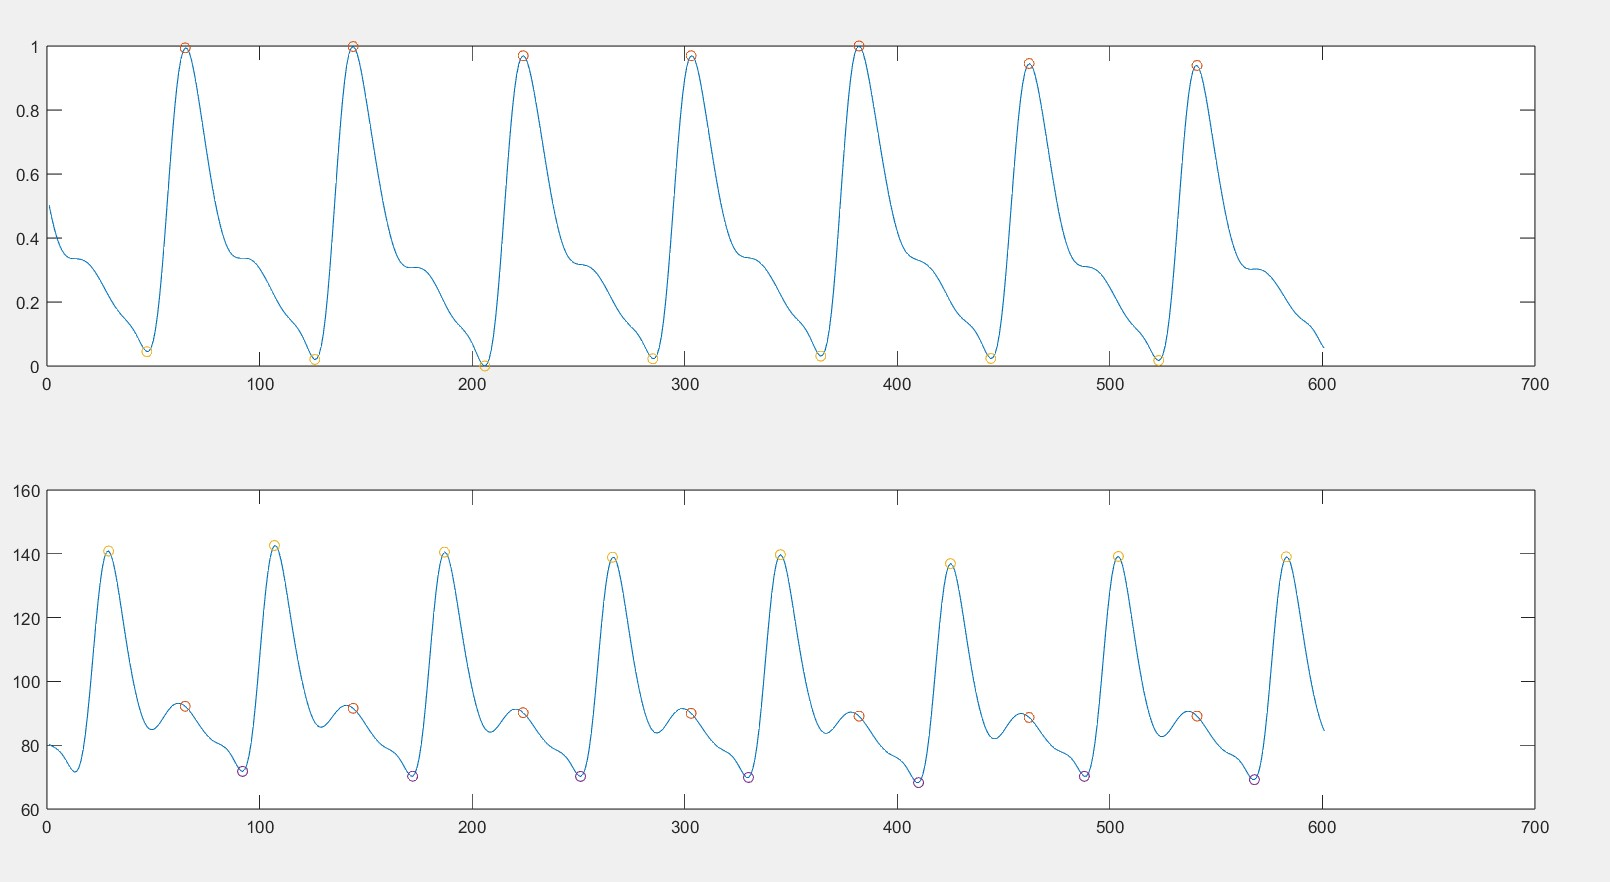
\includegraphics[width=0.4\linewidth]{ImageFiles/data_sample}
		\caption{Esempio di coppia di segnali PPG(in altro) e ABP (in basso).}
		\label{fig:data_sample}
	\end{figure}

	Dopo questa pulizia ho estratto le features seguendo un paper molto noto \cite{6555424}, che ho messo anche su Zotero, risale al 2013 ed è uno dei più citati nel dominio. Quasi tutti i lavori più recenti lo usano come base di partenza. Ci sono diversi modi di estrarre features da un segnale PPG per stimare la pressione sanguigna ma niente di consolidato, è ancora un tema di ricerca.
	
	Una volta estratte le features poi ho fatto un secondo filtraggio, prendendo solo campioni che si riferiscono a valori normali di pressione (sistolica tra 80 e 120, diastolica tra 60 e 100). Questo perché nel dataset ci sono più valori 'normali' di pressione, quelli 'anormali' ci sono in grande numero però si distribuiscono in tanti modi e quindi è come se fossero outliers portando a performance poco buone (MAE di 9 per la sistolica e 6 per la diastolica). Restringendo i campioni a valori di pressione normali è stato sia ridotto il dataset, quindi training più veloce, ma anche performance migliori (MAE di 6 per la sistolica e 3 per la diastolica). Il dataset finale contiene 21801 campioni, ogni campione sono le features estratte da un periodo PPG, ovvero ad un ciclo cardiaco (\Fig~\ref{fig:ppg_hb}). Nel dataset \cite{6555424} ne usano poco più di 15000.
	
	\begin{figure}[h]
		\centering
		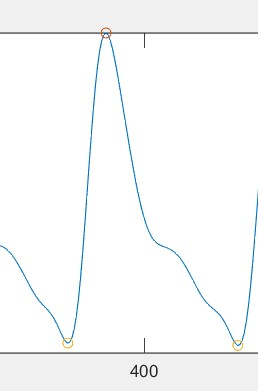
\includegraphics[width=0.7\linewidth]{ImageFiles/ppg_hb}
		\caption{Esempio di un periodo PPG.}
		\label{fig:ppg_hb}
	\end{figure}

	\section{Reti neurali}
	Una volta che i dati erano pronti ho sviluppato due reti neurali usando tensorflow, una MLP e l'atra bayesiana. Ho cercato di tenere un'architettura semplice, più che altro la rete bayesiana poi diventa molto pesante. L'architettura usata è la stessa, due hidden layer: primo da 15 e il secondo da 6 neuroni. Per la BNN ho modellato sia incertezza epistemica che aleatoria.
	
	Ho allenato entrambe le reti con diverse funzioni di costo.
	\begin{itemize}
		\item ANN: MAE, MAPE \\
		\item BNN: MAE, MAPE, NLL (negative log likelihood)
	\end{itemize}

	Sorprendentemente le performance ottenute sono simili tra le due reti con le due reti con tutte le funzioni di costo tranne NLL, dove la bayesiana ha sia MAE che MAPE peggiori. Mi aspettavo risultati peggiori dalla BNN perchè ha veramente molti paramentri in più, 33940 contro i 350 della ANN.
	
	
	\section{Robustezza}
	Ho fatto una prima analisi di robustezza seguendo un po' quello che era stato fatto della tesi precedente. Ho usato solo il rumore gaussiano bianco come alterazione, come range ho usato una deviazione standard da 0 a 2, con step di 0.1. Sembra basso ma in realtà i segnali PPG hanno ampiezze molto piccole e già con 1 il segnale è parecchio perturbato.
	
	Dopo sul dataset alterato ho fatto le predizioni e calcolato le metriche di interesse. In particolare il MAE insieme alle formule discusse l'ultima volta (\Eq~\ref{eff1},\Eq~\ref{eff2}), che misurano 'l'infefficienza' della rete. Come misura di incertezza ho usato la larghezza dell'intervallo di confidenza al 95\%.
	
	\begin{equation}
		\label{eff1}
		ineff1 = \frac{\sigma}{error + 1} + \frac{error}{\sigma + 1}
	\end{equation}
	\begin{equation}
		\label{eff2}
		ineff2 = \frac{\sigma + 1}{error + 1} + \frac{error + 1}{\sigma + 1}
	\end{equation}
	
	\subsection{Analisi BNN con MAE}
	In figura ~\ref{fig:mae_bnn} ci sono i grafici con i risultati, la linea rossa in ciascuno di essi indica le condizioni nominali.
	
	\begin{figure}[h]
		\centering
		\begin{subfigure}{.5\textwidth}
			\centering
			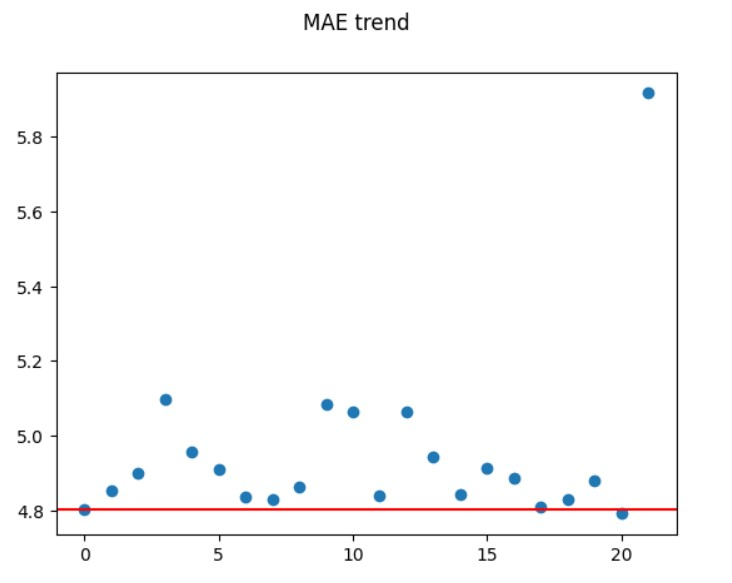
\includegraphics[width=0.7\linewidth]{ImageFiles/mae_bnn_mae}
			\caption{}
			\label{fig:mae_bnn_mae}
		\end{subfigure}%
		\begin{subfigure}{.5\textwidth}
			\centering
			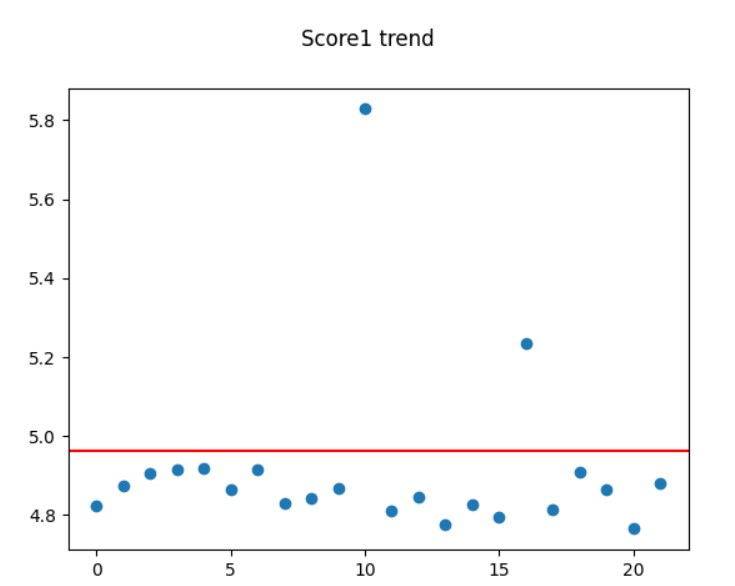
\includegraphics[width=0.7\linewidth]{ImageFiles/mae_bnn_eff1}
			\caption{}
			\label{fig:mae_bnn_eff1}
		\end{subfigure}
	
		\begin{subfigure}{.5\textwidth}
			\centering
			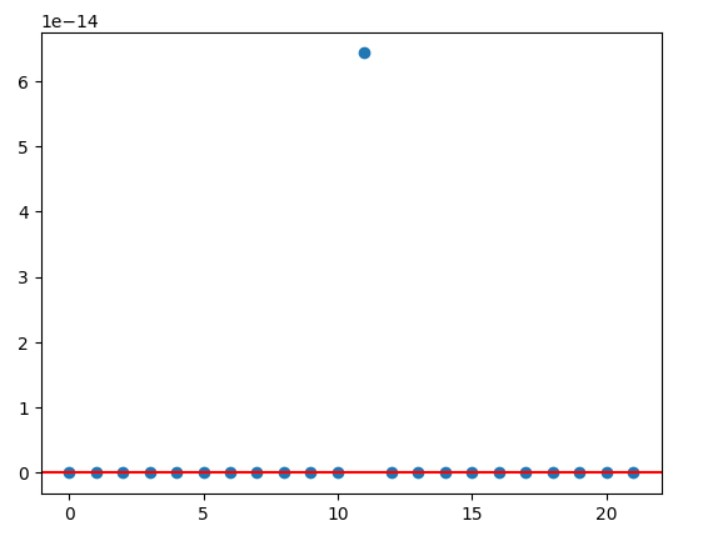
\includegraphics[width=0.7\linewidth]{ImageFiles/mae_bnn_ci}
			\caption{}
				\label{fig:mae_bnn_ci}
		\end{subfigure}%
		\begin{subfigure}{.5\textwidth}
			\centering
			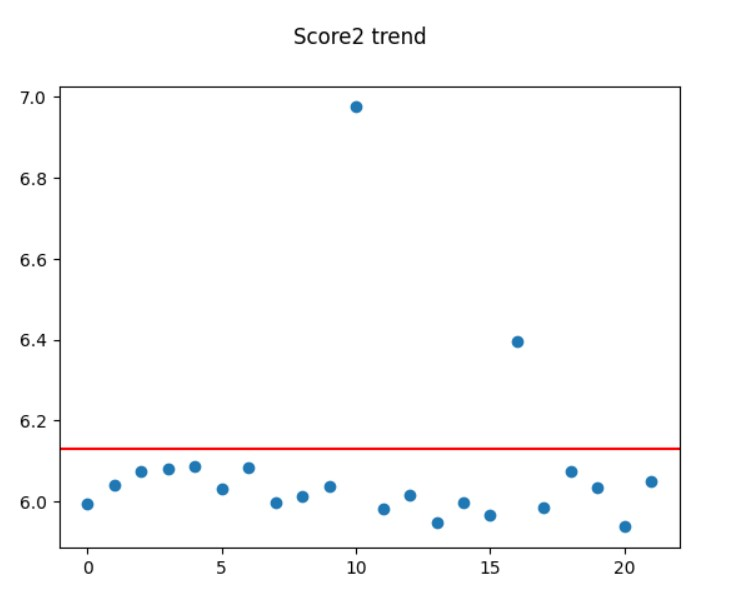
\includegraphics[width=0.7\linewidth]{ImageFiles/mae_bnn_eff2}
			\caption{}
			\label{fig:mae_bnn_eff2}
		\end{subfigure}
		\caption{Risultati predizioni sul test set alterato per la BNN con MAPE.}
		\label{fig:mae_bnn}
	\end{figure}

	Guardando questi grafici sembrerebbe che la rete sia molto robusta, cioè tolti alcuni picchi (cosa strana) poi il resto si comporta bene, è molto vicina alle condizioni nominali. Per c'è anche da dire che le BNN sono note per la robustezza al rumore gaussiano grazie alla loro natura stocastica.
	
	\subsection{Analisi BNN con MAPE}
	In figura ~\ref{fig:mape_bnn} ci sono i grafici come prima. Di nuovo sembrerebbe che si comporti abbastanza bene. Però l'incertenza sembra essere sempre e bassa, tranne in un paio di casi, e questo potrebbe essere un comportamento poco desiderato.
	
	\begin{figure}[h]
		\centering
		\begin{subfigure}{.5\textwidth}
			\centering
			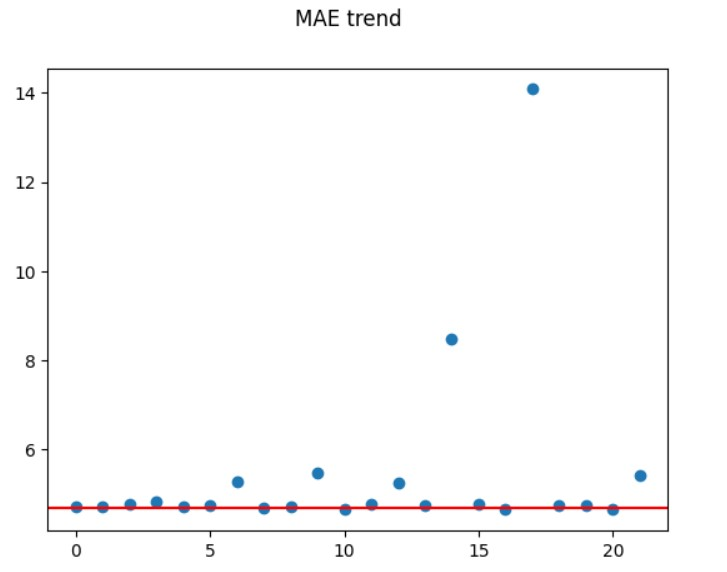
\includegraphics[width=0.7\linewidth]{ImageFiles/mape_bnn_mae}
			\caption{}
			\label{fig:mape_bnn_mae}
		\end{subfigure}%
		\begin{subfigure}{.5\textwidth}
			\centering
			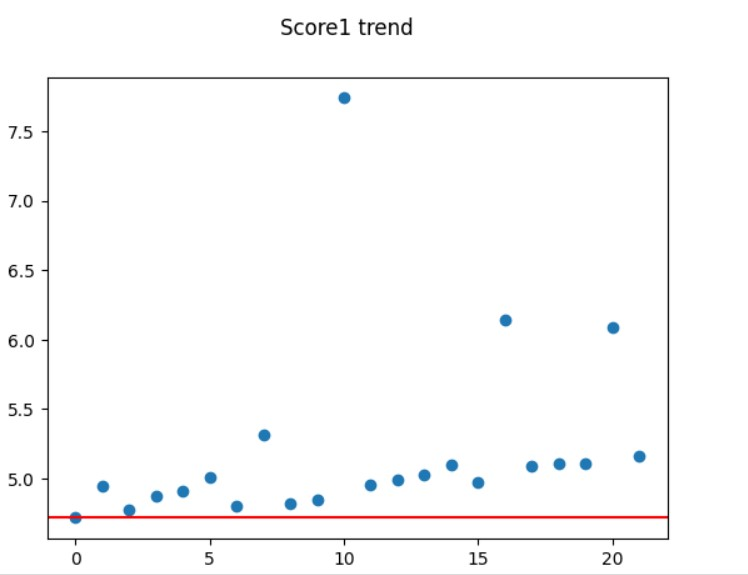
\includegraphics[width=0.7\linewidth]{ImageFiles/mape_bnn_eff1}
			\caption{}
			\label{fig:mape_bnn_eff1}
		\end{subfigure}
		\begin{subfigure}{.5\textwidth}
			\centering
			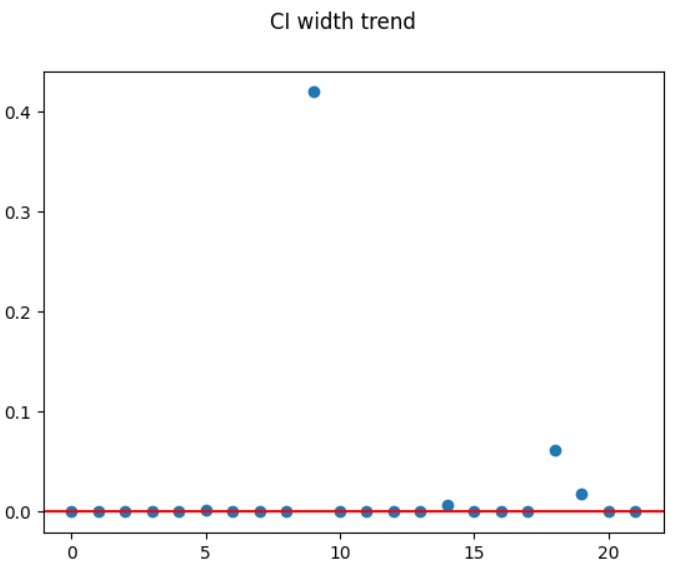
\includegraphics[width=0.7\linewidth]{ImageFiles/mape_bnn_ci}
			\caption{}
			\label{fig:mape_bnn_ci}
		\end{subfigure}%
		\begin{subfigure}{.5\textwidth}
			\centering
			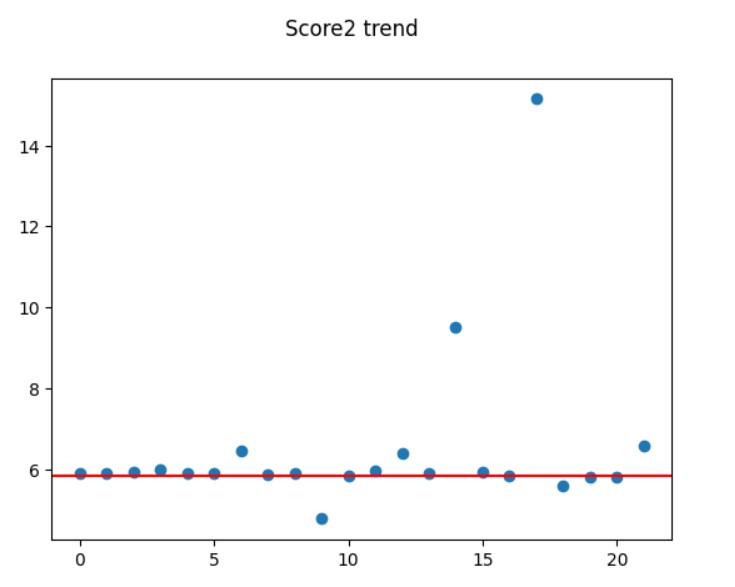
\includegraphics[width=0.7\linewidth]{ImageFiles/mape_bnn_eff2}
			\caption{}
			\label{fig:mae_bnn_eff2}
		\end{subfigure}
		\caption{Risultati predizioni sul test set alterato per la BNN con MAPE.}
		\label{fig:mape_bnn}
	\end{figure}
	
	\subsection{Analisi BNN con NLL}
	In questo caso ci sono risultati più interessanti. La rete si comporta molto male a livello di MAE, cosa che era attendibile visto che già in fase di traning aveva un MAE basso. In figura ~\ref{fig:nll_bnn} ci sono 4 grafici che mostrano questo comportamento. La cosa sorprendente è che fa molto meglio in termini di eff1 ed eff2 rispetto alle condizioni nominali e questo mi sembra più curioso.
	
	\begin{figure}[h]
		\centering
		\begin{subfigure}{.5\textwidth}
			\centering
			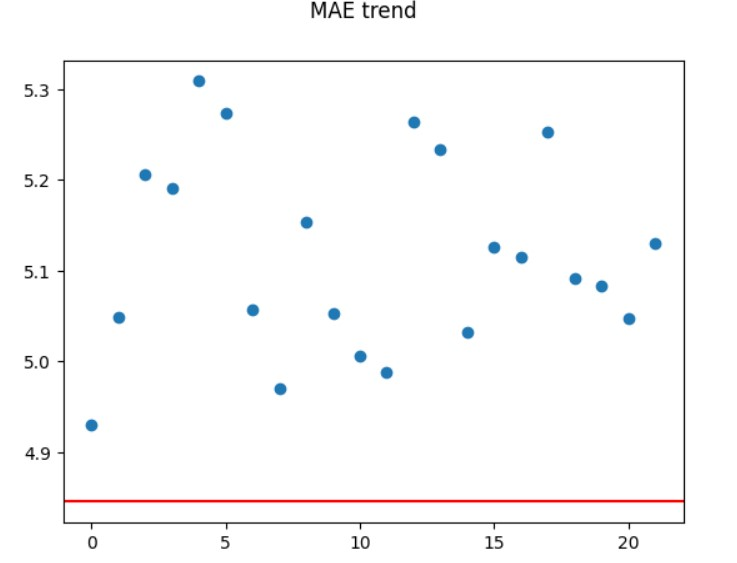
\includegraphics[width=0.7\linewidth]{ImageFiles/nll_bnn_mae}
			\caption{}
			\label{fig:nll__bnn_mae}
		\end{subfigure}%
		\begin{subfigure}{.5\textwidth}
			\centering
			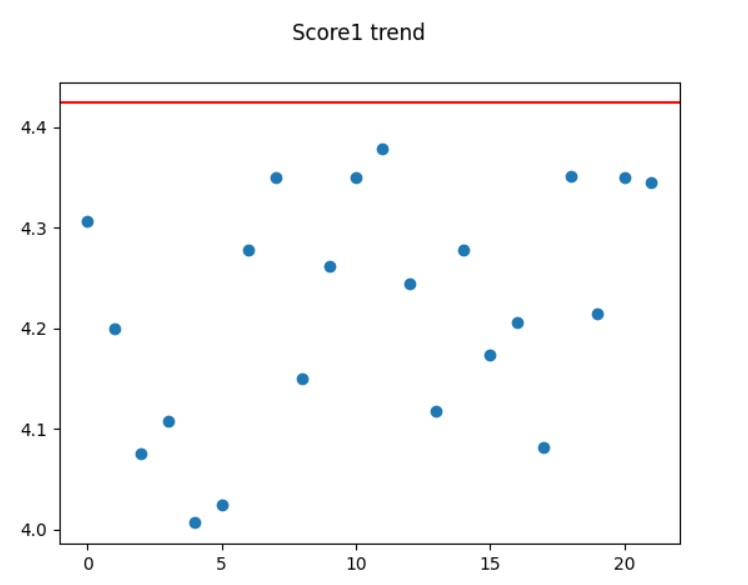
\includegraphics[width=0.7\linewidth]{ImageFiles/nll_bnn_eff1}
			\caption{}
			\label{fig:nll_bnn_eff1}
		\end{subfigure}
	
		\begin{subfigure}{.5\textwidth}
			\centering
			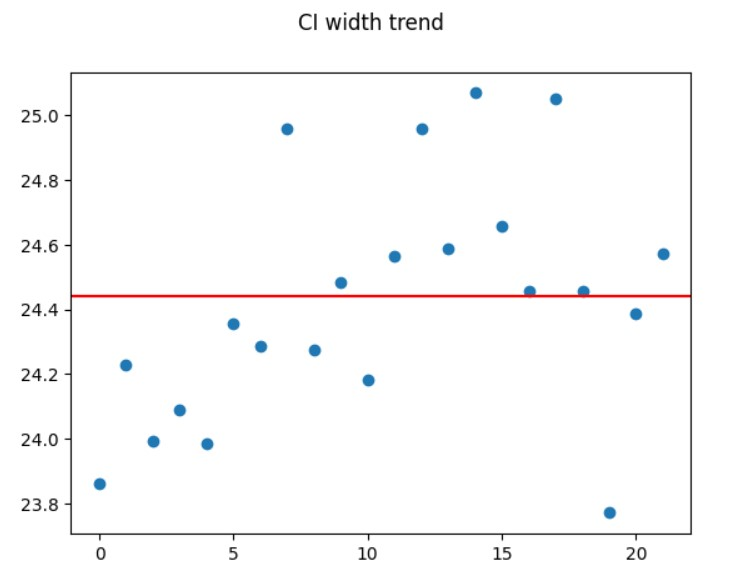
\includegraphics[width=0.7\linewidth]{ImageFiles/nll_bnn_ci}
			\caption{}
			\label{fig:nll_bnn_ci}
		\end{subfigure}%
		\begin{subfigure}{.5\textwidth}
			\centering
			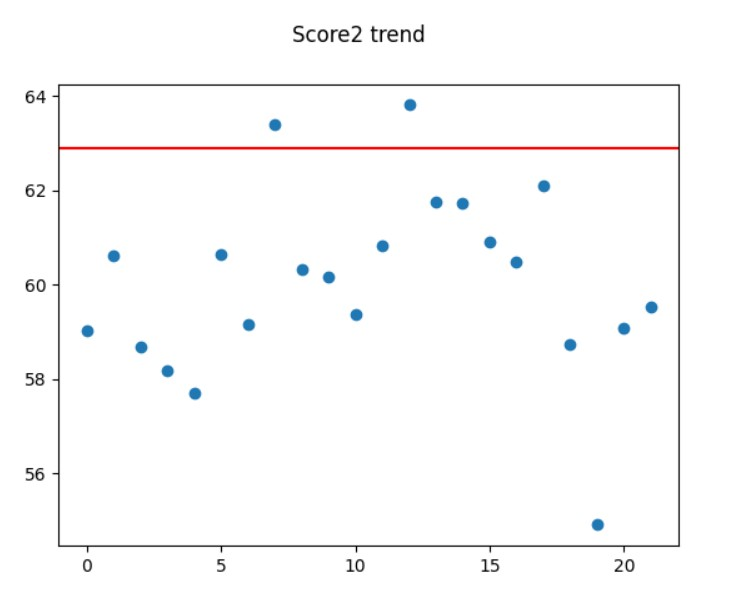
\includegraphics[width=0.7\linewidth]{ImageFiles/nll_bnn_eff2}
			\caption{}
			\label{fig:nll_bnn_eff2}
		\end{subfigure}
		\caption{Risultati predizioni sul test set alterato per la BNN con NLL.}
		\label{fig:nll_bnn}
	\end{figure}

	Ovviamente queste sono solo prime analisi fatte e sarebbe da investigare meglio, però visto che sono i primi risultati concreti valeva la pena analizzarli.
	
	\subsection{Considerazioni teoriche}
	Le due formule \Eq~\ref{eff1} ed \Eq~\ref{eff2} misurano una sorta di inefficienza della rete. Le due formule sembrerebbe che si comportino in modo molto simile, tranne per il fatto che \Eq~\ref{eff2} può essere invertita senza problema, quindi essere usata come misura di bontà. Però forse non è tanto utile come cosa, nel senso che tutte le metriche su reti neurali tendono a valutare quanto la rete performa male e non il viceversa. Tra due \Eq~\ref{eff1} secondo me ha più senso, anche se non invertibile. Ha senso perché è come se fosse un'estensione dell'errore classico, ovvero mettendosi nel caso deterministico con $\sigma=0$ di ritorna ad avere solo la misura di errore, cosa che ne giustifica l'utilizzo. Poi anche il suo andamento è più 'deciso' nei primi tratti partendo da (0,0) per poi essere più smooth dopo, cosa che ha senso perché premia di più l'intorno (0,0), che è il punto ideale.
	
	
	\clearpage
	
	\bibliographystyle{ieeetr}
	
	\bibliography{./OtherFiles/Bibliography}
	
	\addcontentsline{toc}{section}{Bibliography}
	
\end{document}